\section{Results}
\label{sec:performanceTestResults}
\begin{figure}[t]
    \centering
    \captionsetup{justification=centering, format=hang}
    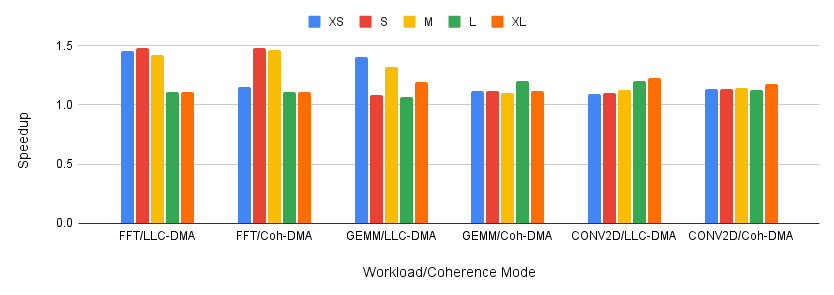
\includegraphics[width=1\linewidth]{fig/DMA_chart.png}
    \caption{Accelerator memory access speedup provided by the pipelined LLC for for various applications and workload sizes.}
    \label{fig:dma_chart}
\end{figure}

To characterize the performance improvements pipelining the LLC provides, we
generated FPGA bitstreams of ESP SoCs with 256KB configurations of both
implementations. Each SoC features 3 different types of accelerators: Fast
Fourier Transform (FFT), General Matrix Multiply (GEMM), and 2D Convolution
(CONV2D). We ran baremetal applications to invoke each accelerator across a
range of workload sizes from a several KB (XS) to a few MB (XL).  To
focus on the performance of the LLC, we used two different modes of accelerator
coherence that access data from the LLC: LLC-coherent DMA (LLC-DMA)
requires a flush of the private L2 caches to ensure data is in the LLC before an
accelerator starts, while Coherent-DMA (Coh-DMA) does not require a flush and
potentially has to recall modified cache lines from private L2s. We leveraged
the ESP hardware monitors API to measure the number of cycles that the
accelerator spends communicating with the memory hierarchy and the total number
of execution cycles.

\par Figure \ref{fig:dma_chart} shows the speedup that the pipelined LLC
provides for memory accesses from the accelerator.  While the speedup for
CONV2D stays relatively constant across different workloads, the speedup is
much larger for FFT and GEMM at smaller to medium workloads. Larger workloads
do not fit in the LLC, so most of the accelerator data will be in off-chip
memory, limiting the improvements of the pipelined LLC. The memory access
speedup ranges from 7\% to 48\%, with an average of 20\%. This results in
speedups of the entire accelerator execution as as high as 10\% and 2\% on
average.

We validated our pipelined implementation further by booting a Linux OS on the
RISC-V core of the SoC and plan to test and characterize multicore SoCs in the
near future. We plan to make our implementation of the pipelined LLC available
as open-source hardware as part of the next ESP public release.
